\documentclass[a4paper,12pt]{article}
\usepackage{amsmath, amssymb, amsthm, color, graphicx}
\usepackage{xcolor}

\definecolor{rojo}{RGB}{200, 0, 0}
\definecolor{azul}{RGB}{0, 0, 200}
\definecolor{verde}{RGB}{0, 150, 0}
\definecolor{naranja}{RGB}{255, 140, 0}
\definecolor{resaltado}{RGB}{220, 220, 220}

\begin{document}

\section*{Solución al Problema 1}

\subsection*{1. Construcción del espacio de probabilidad \((\Omega, \mathcal{F}, P)\)}

El espacio muestral es:
\[
\Omega = \{ \textcolor{rojo}{\text{rojo}}, \textcolor{azul}{\text{azul}}, \textcolor{verde}{\text{verde}}, \textcolor{naranja}{\text{naranja}} \}.
\]

La \(\sigma\)-álgebra de eventos es:
\[
\mathcal{F} = 2^\Omega.
\]
\textit{Disclaimer: Como nos ha dicho Hugo en la ayudantía cada vez que tenemos un espacio muestral de dimensión finita el $\sigma-algebra$ de eventos es el conjunto potencia.}


La función de probabilidad \(P: \mathcal{F} \to [0,1]\) se define como:
\[
P(\{\textcolor{rojo}{\text{rojo}}\}) = \frac{2}{8}, \quad
P(\{\textcolor{azul}{\text{azul}}\}) = \frac{3}{8}, \quad
P(\{\textcolor{verde}{\text{verde}}\}) = \frac{1}{8}, \quad
P(\{\textcolor{naranja}{\text{naranja}}\}) = \frac{2}{8}.
\]

\subsection*{2. Definición de la variable aleatoria \(X: \Omega \to \mathbb{R}\)}

Definimos una variable aleatoria asignando valores numéricos a los colores:
\[
X(\textcolor{rojo}{\text{rojo}}) = 1, \quad
X(\textcolor{azul}{\text{azul}}) = 2, \quad
X(\textcolor{verde}{\text{verde}}) = 3, \quad
X(\textcolor{naranja}{\text{naranja}}) = 4.
\]

\subsection*{3. Función de probabilidad y función de distribución}

La función de probabilidad \(P_X\) es:
\[
P_X(1) = \frac{2}{8}, \quad
P_X(2) = \frac{3}{8}, \quad
P_X(3) = \frac{1}{8}, \quad
P_X(4) = \frac{2}{8}.
\]

La función de distribución \(F_X(x) = P(X \leq x)\) es:

\[
F_X(x) =
\begin{cases}
0, & x < 1, \\
\frac{2}{8}, & 1 \leq x < 2, \\
\frac{5}{8}, & 2 \leq x < 3, \\
\frac{6}{8}, & 3 \leq x < 4, \\
1, & x \geq 4.
\end{cases}
\]

\subsection*{4. Esperanza y varianza}

Calculamos la esperanza:

\[
E[X] = \sum_{x} x P_X(x) = 1 \cdot \frac{2}{8} + 2 \cdot \frac{3}{8} + 3 \cdot \frac{1}{8} + 4 \cdot \frac{2}{8}.
\]

\[
E[X] = \frac{2}{8} + \frac{6}{8} + \frac{3}{8} + \frac{8}{8} = \frac{19}{8} = 2.375.
\]

Ahora, calculamos \(E[X^2]\):

\[
E[X^2] = 1^2 \cdot \frac{2}{8} + 2^2 \cdot \frac{3}{8} + 3^2 \cdot \frac{1}{8} + 4^2 \cdot \frac{2}{8}.
\]

\[
E[X^2] = \frac{2}{8} + \frac{12}{8} + \frac{9}{8} + \frac{32}{8} = \frac{55}{8} = 6.875.
\]

La varianza es:

\[
\text{Var}(X) = E[X^2] - (E[X])^2.
\]

\[
\text{Var}(X) = 6.875 - (2.375)^2 = 6.875 - 5.6406 = 1.2344.
\]

\section*{Solución al Problema 2}

Queremos construir una \(\sigma\)-álgebra \(\mathcal{G}\) que contenga \(A\) pero que no sea la \(\sigma\)-álgebra discreta.

Sea:

\[
\Omega = \{ \omega_1, \omega_2, \omega_3, \omega_4 \},
\]

y un conjunto particular \(A\):

\[
A = \{ \omega_1, \omega_2 \}.
\]

Para formar una \(\sigma\)-álgebra válida, debemos incluir:
\begin{itemize}
    \item El conjunto vacío: \(\emptyset\).
    \item El conjunto dado: \(A = \{ \omega_1, \omega_2 \}\).
    \item Su complemento: \(A^c = \{ \omega_3, \omega_4 \}\).
    \item El espacio muestral completo: \(\Omega\).
\end{itemize}

Por lo tanto, una \(\sigma\)-álgebra que satisface la condición pedida es:

\[
\mathcal{G} = \{ \emptyset, A, A^c, \Omega \}.
\]

Esta es una \(\sigma\)-álgebra propiamente contenida en \(2^\Omega\), lo que prueba que \(\mathcal{G} \neq 2^\Omega\), cumpliendo así con la condición de no ser la \(\sigma\)-álgebra discreta.

\section*{Solución al Problema 3}

\begin{figure}[h]
    \centering
    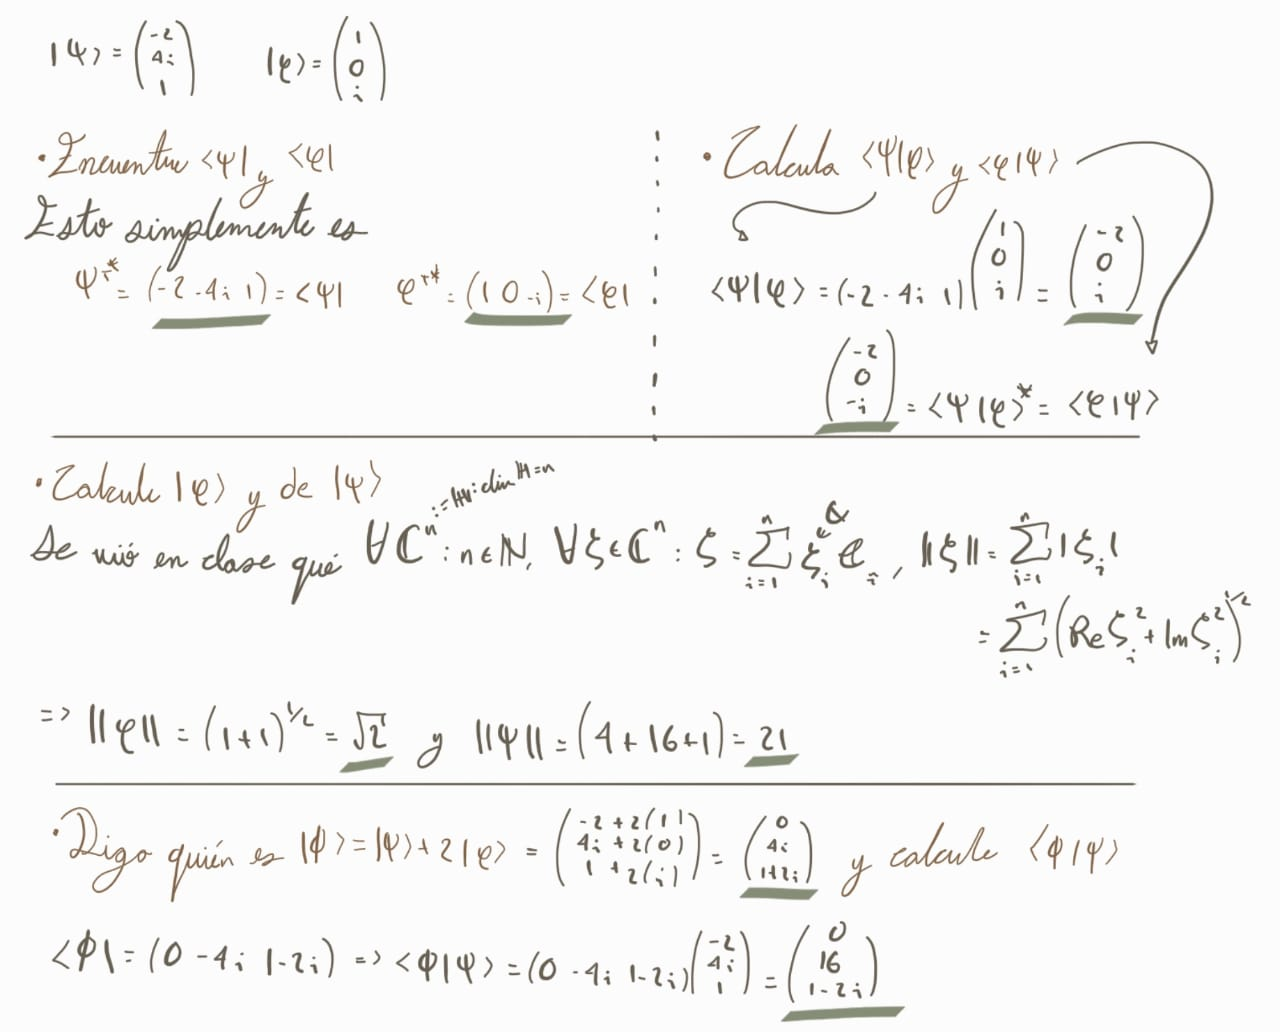
\includegraphics[width=1\linewidth]{tablet.jpg}
    \label{fig:enter-label}
\end{figure}

\section*{Solución al Problema 4}
Es la funcional lineal Bra

\newpage
\section*{Solución al Problema 5}

Sea $\mathcal{H}$ un espacio de Hilbert sobre $\mathbb{C}$ con producto escalar
$\langle \cdot \mid \cdot \rangle$ y sea $A : \mathcal{H} \to \mathcal{H}$ un operador
(lineal). Demostrar que:
$\text{(a)}\quad (A^*)^* = A, \quad$ \\
$\text{(b)}\quad (cA)^* = \overline{c}\, A^* \text{ para todo } c \in \mathbb{C}, \quad$ \\
$\text{(c)}\quad \langle A \rangle = \langle \psi \mid A\phi\rangle^*, \quad$ \\
$\text{(d)}\quad \bigl(\lvert\psi\rangle\langle\phi\rvert\bigr)^* = \lvert\phi\rangle\langle\psi\rvert.$ \\

\textcolor{red}{\subsection*{(a) Prueba de $(A^*)^* = A$}}

\noindent
\textcolor{purple}{
Para ver que $(A^*)^* = A$, basta verificar que para cualesquiera
$\lvert \psi \rangle, \lvert \phi \rangle \in \mathcal{H}$ se cumpla:
\[
\langle (A^*)^* \psi \mid \phi \rangle \;=\; \langle \psi \mid A \phi \rangle.
\]
}
\textcolor{black}{
En efecto, por definición de adjunto, $A^*$ es el único operador tal que
\[
\langle A^* \psi \mid \phi \rangle \;=\; \langle \psi \mid A \phi \rangle
\quad \text{para todo } \lvert \psi\rangle, \lvert \phi\rangle.
\]
Entonces, si definimos $B := (A^*)^*$, se verifica que
\[
\langle B \psi \mid \phi \rangle 
\;=\; \langle (A^*)^* \psi \mid \phi \rangle
\;=\; \langle \psi \mid A \phi \rangle,
\]
lo cual es precisamente la caracterización de $A$. Por unicidad del adjunto,
obtenemos $B = A$, es decir, $(A^*)^* = A$.
}

\vspace{1em}

\textcolor{red}{\subsection*{(b) Prueba de $(cA)^* = \overline{c}\, A^*$}}

\noindent
\textcolor{purple}{
Sea $c \in \mathbb{C}$. Observemos que para todo $\lvert \psi\rangle, \lvert \phi\rangle \in \mathcal{H}$,
\[
\langle (cA)^* \psi \mid \phi \rangle 
\;=\; \langle \psi \mid cA \phi \rangle 
\;=\; c \, \langle \psi \mid A \phi \rangle.
\]
}
\textcolor{black}{
Sin embargo, por definición de adjunto, si $B = (cA)^*$, entonces
\[
\langle B \psi \mid \phi \rangle
\;=\; \langle \psi \mid cA \phi \rangle
\;=\; c\, \langle \psi \mid A \phi \rangle.
\]
Por otra parte, 
\[
\langle \overline{c}\, A^* \psi \mid \phi \rangle
\;=\; \overline{c}\,\langle A^* \psi \mid \phi \rangle
\;=\; \overline{c}\,\langle \psi \mid A \phi \rangle
\;=\; c\, \langle \psi \mid A \phi \rangle,
\]
donde en el último paso se ha usado que $\overline{c} \cdot \langle \psi \mid A \phi \rangle
= c \cdot \langle \psi \mid A \phi \rangle$ cuando pasamos el conjugado complejo fuera
del producto escalar de manera adecuada (y considerando que $c \in \mathbb{C}$ puede ser reescrito en su forma conjugada en el lado correspondiente, \textcolor{purple}{anticonmutatividad}).
Comparando ambos resultados, deducimos $(cA)^* = \overline{c}\, A^*$.
}

\vspace{1em}

\textcolor{red}{\subsection*{(c) Prueba de $\langle A \rangle = \langle \psi \mid A \phi\rangle^*$}}

\noindent
En el contexto de las aplicaciones lineales duales, si definimos las aplicaciones
\[
M_\psi : \mathcal{H} \to \mathbb{C}, \quad \lvert \phi \rangle \mapsto \langle \psi \mid \phi\rangle,
\]
\[
M_\psi^A : \mathcal{H} \to \mathbb{C}, \quad \lvert \phi \rangle \mapsto \langle \psi \mid A\phi\rangle,
\]
entonces la regla de adjunto implica que
\[
\langle A \rangle \;=\; \langle \psi \mid A\phi\rangle^*
\]
bajo la interpretación de que $\langle A \rangle$ corresponde a la forma sesquilineal
resultante de aplicar $A$ y luego tomar producto escalar.

\vspace{1em}

\textcolor{red}{\subsection*{(d) Prueba de $\bigl(\lvert\psi\rangle\langle\phi\rvert\bigr)^* = \lvert\phi\rangle\langle\psi\rvert$}}

\noindent
Recordemos la Definición 2.8 del adjunto de un operador y consideremos
$|\psi\rangle\langle\phi|: \mathcal{H} \to \mathcal{H}$. Para todo
$\lvert \eta\rangle, \lvert \xi\rangle \in \mathcal{H}$,
\[
\langle (|\psi\rangle\langle\phi|)\,\eta \mid \xi \rangle
\;=\; \langle\phi|\eta\rangle \, \langle \psi \mid \xi\rangle.
\]
\textcolor{purple}{
En cambio, 
\[
\langle \eta \mid (|\psi\rangle\langle\phi|)^* \,\xi \rangle
\;=\; \overline{\langle (|\psi\rangle\langle\phi|)\,\eta \mid \xi \rangle}
\;=\; \overline{\langle\phi|\eta\rangle \, \langle \psi \mid \xi\rangle}
\;=\; \langle \eta \mid \phi\rangle \, \overline{\langle \psi \mid \xi\rangle}.
\]
}
\textcolor{black}{
Observamos que
\[
\langle \eta \mid \phi\rangle \, \overline{\langle \psi \mid \xi\rangle}
\;=\; \langle \eta \mid \phi\rangle \, \langle \xi \mid \psi\rangle
\;=\; \langle \eta \mid \phi\rangle \langle \xi \mid \psi\rangle.
\]
Por la definición de $|\phi\rangle\langle\psi|$, se tiene
\[
|\phi\rangle\langle\psi|\;:\;\lvert \xi\rangle \;\mapsto\; \langle\psi|\xi\rangle \,\lvert \phi\rangle,
\]
y entonces
\[
\langle \eta \mid (|\phi\rangle\langle\psi|)\,\xi \rangle
\;=\; \langle \eta \mid \langle\psi|\xi\rangle\, \phi \rangle
\;=\; \langle\psi|\xi\rangle \, \langle \eta \mid \phi\rangle,
\]
que coincide con la expresión anterior. Por unicidad del adjunto concluimos
\[
\bigl(|\psi\rangle\langle\phi|\bigr)^* \;=\; |\phi\rangle\langle\psi|.
\]
}

\newpage
\section*{Solución al Problema 6}
\begin{figure}[h]
    \centering
    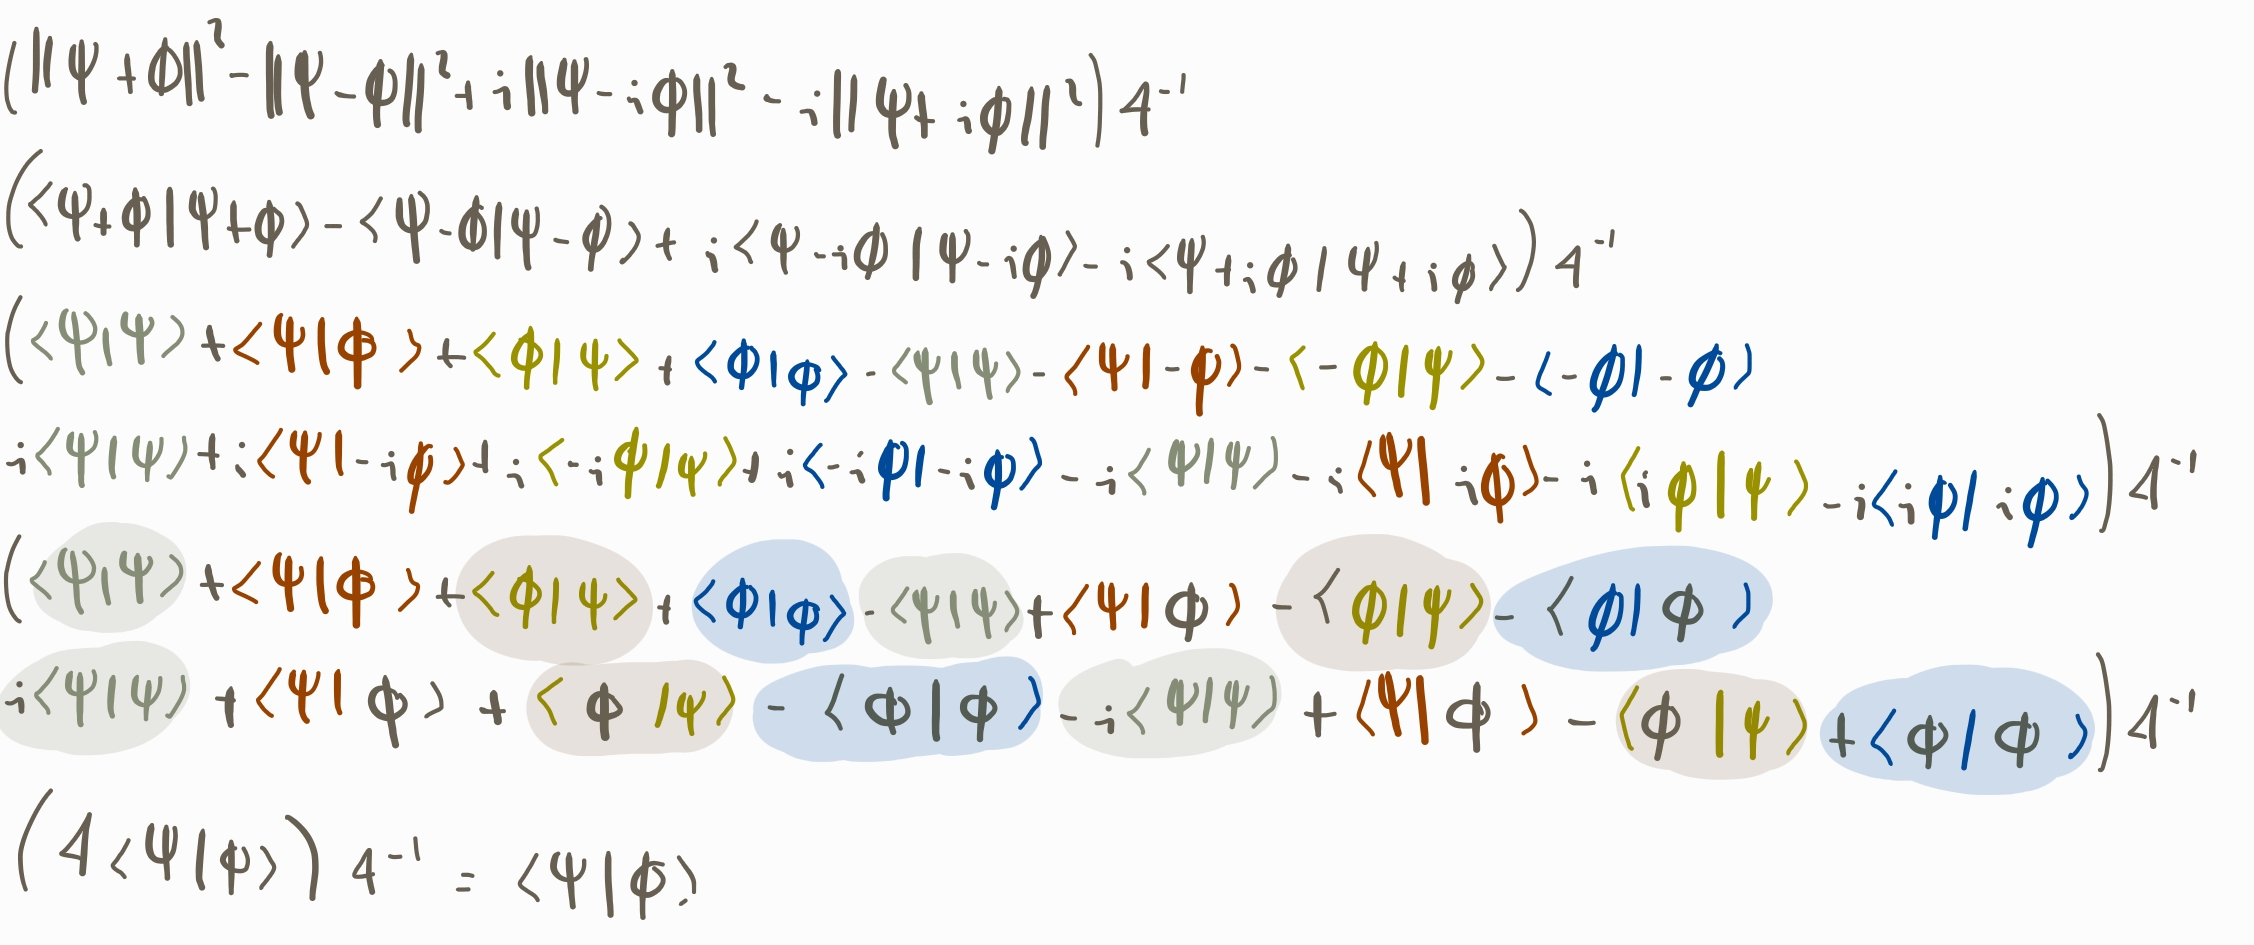
\includegraphics[width=1\linewidth]{polarizacion.jpg}
\end{figure}

\section{Solución al Problema 7}
Trivial (en realidad no tengo idea, lo siento :c)

\end{document}
